\documentclass{beamer}
\mode<presentation>
\usepackage{amsmath}
\usepackage{amssymb}
%\usepackage{advdate}
\usepackage{adjustbox}
\usepackage{subcaption}
\usepackage{enumitem}
\usepackage{multicol}
\usepackage{gensymb}
\usepackage{mathtools}
\usepackage{listings}
\usepackage{url}
\def\UrlBreaks{\do\/\do-}
\usetheme{Boadilla}
\usecolortheme{lily}
\setbeamertemplate{footline}
{
  \leavevmode%
  \hbox{%
  \begin{beamercolorbox}[wd=\paperwidth,ht=2ex,dp=1ex,right]{author in head/foot}%
    \insertframenumber{} / \inserttotalframenumber\hspace*{2ex} 
  \end{beamercolorbox}}%
  \vskip0pt%
}
\setbeamertemplate{navigation symbols}{}

\providecommand{\nCr}[2]{\,^{#1}C_{#2}} % nCr
\providecommand{\nPr}[2]{\,^{#1}P_{#2}} % nPr
\providecommand{\mbf}{\mathbf}
\providecommand{\pr}[1]{\ensuremath{\Pr\left(#1\right)}}
\providecommand{\qfunc}[1]{\ensuremath{Q\left(#1\right)}}
\providecommand{\sbrak}[1]{\ensuremath{{}\left[#1\right]}}
\providecommand{\lsbrak}[1]{\ensuremath{{}\left[#1\right.}}
\providecommand{\rsbrak}[1]{\ensuremath{{}\left.#1\right]}}
\providecommand{\brak}[1]{\ensuremath{\left(#1\right)}}
\providecommand{\lbrak}[1]{\ensuremath{\left(#1\right.}}
\providecommand{\rbrak}[1]{\ensuremath{\left.#1\right)}}
\providecommand{\cbrak}[1]{\ensuremath{\left\{#1\right\}}}
\providecommand{\lcbrak}[1]{\ensuremath{\left\{#1\right.}}
\providecommand{\rcbrak}[1]{\ensuremath{\left.#1\right\}}}
\theoremstyle{remark}
\newtheorem{rem}{Remark}
\newcommand{\sgn}{\mathop{\mathrm{sgn}}}
\providecommand{\abs}[1]{\left\vert#1\right\vert}
\providecommand{\res}[1]{\Res\displaylimits_{#1}} 
\providecommand{\norm}[1]{\lVert#1\rVert}
\providecommand{\mtx}[1]{\mathbf{#1}}
\providecommand{\mean}[1]{E\left[ #1 \right]}
\providecommand{\fourier}{\overset{\mathcal{F}}{ \rightleftharpoons}}
%\providecommand{\hilbert}{\overset{\mathcal{H}}{ \rightleftharpoons}}
\providecommand{\system}{\overset{\mathcal{H}}{ \longleftrightarrow}}
	%\newcommand{\solution}[2]{\textbf{Solution:}{#1}}
%\newcommand{\solution}{\noindent \textbf{Solution: }}
\providecommand{\dec}[2]{\ensuremath{\overset{#1}{\underset{#2}{\gtrless}}}}
\newcommand{\myvec}[1]{\ensuremath{\begin{pmatrix}#1\end{pmatrix}}}
\let\vec\mathbf

\lstset{
%language=C,
frame=single, 
breaklines=true,
columns=fullflexible
}

\numberwithin{equation}{section}

\title{10.3.2.4.4 Presentation}
\author{G. Abhimanyu Koushik \\ EE24BTECH11024}

\date{\today} 
\begin{document}

\begin{frame}
\titlepage
\end{frame}

\section*{Outline}
\begin{frame}
\tableofcontents
\end{frame}
\section{Problem}
\begin{frame}
\frametitle{Problem Statement}
%
Check is the pair of linear equations $2x-2y-2=0$, $4x-4y-5=0$. And if consistent, obtain the solution
%
\end{frame}

%\subsection{Literature}
\section{Solution}
\begin{frame}
\frametitle{Solution}
%\framesubtitle{Literature}
Given
\begin{align}
    2x-2y-2=0\\
    4x-4y-5 = 0
\end{align}
Simplifying and using matrix notation,
\begin{align}
    \myvec{
        1 & -1\\
        4 & -4
    } \myvec{x \\ y}= \myvec{ 1 \\ 5}
\end{align}
\end{frame}
\begin{frame}
The matrix $A$ can be decomposed into:
\begin{align}
    A = L \cdot U,
\end{align}
where:
\begin{align}
    L &= \myvec{1 & 0 \\ 4 & 1}, \\
    U &= \myvec{1 & -1 \\ 0 & 0}.
\end{align}
\newline
\end{frame}
\begin{frame}
Factorization of LU:\newline
Given a matrix $ \mathbf{A} $ of size $ n \times n $, LU decomposition is performed row by row and column by column. The update equations are as follows: \\ 
\qquad 1. Start by initializing $ \mathbf{L} $ as the identity matrix $ \mathbf{L} = \mathbf{I} $ and $ \mathbf{U} $ as a copy of $ \mathbf{A} $.\\
\qquad 2. For each column $ j \geq k $, the entries of $ U $ in the $ k $-th row are updated as:
\begin{align}
U_{k,j} = A_{k,j} - \sum_{m=1}^{k-1} L_{k,m} \cdot U_{m,j}\quad \forall \quad j \geq k
\end{align}
3. For each row $ i > k $, the entries of $ L $ in the $ k $-th column are updated as:
\begin{align}
L_{i,k} = \frac{1}{U_{k,k}} \brak{ A_{i,k} - \sum_{m=1}^{k-1} L_{i,m} \cdot U_{m,k}} \quad \forall \quad i > k
\end{align}
\end{frame}
\begin{frame}
The system $A\vec{x} = \vec{b}$ is transformed into $L \cdot U \cdot \vec{x} = \vec{b}$. Let $\vec{y}$ satisfy $L\vec{y} = \vec{b}$:
\begin{align}
    \myvec{1 & 0 \\ 4 & 1} \myvec{y_1 \\ y_2} = \myvec{1 \\ 5}.
\end{align}
Using forward substitution:
\begin{align}
    y_1 &= 1 \\
    4y_1 + y_2 &= 5\\
    y_2 &= 1
\end{align}
Thus:
\begin{align}
    \vec{y} = \myvec{1 \\ 1}.
\end{align}
\end{frame}
\begin{frame}
Next, solve $U\vec{x} = \vec{y}$:
\begin{align}
    \myvec{1 & -1 \\ 0 & 0} \myvec{x \\ y} = \myvec{1 \\ 1}.
\end{align}

Using back substitution:
\begin{align}
	0x+0y = 1
\end{align}
As it is not possible for any value of $x$ and $y$, the solution does not exist.
\end{frame}
\section{Plot}
\begin{frame}
\frametitle{Plot}
\begin{figure}[h!]
   \centering
   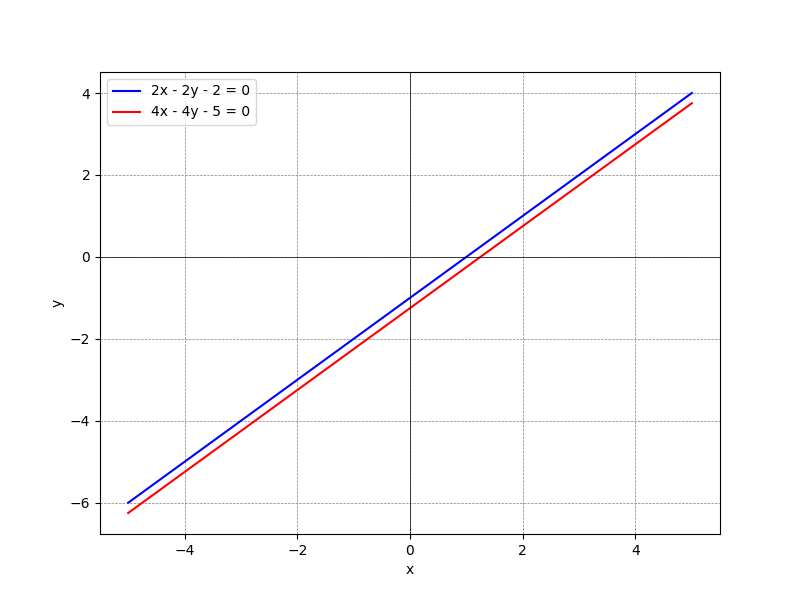
\includegraphics[width=0.8\columnwidth]{figs/fig.png}
   \caption{Graph of the given lines}
   \label{stemplot}
\end{figure}
\end{frame}
\end{document}

